\section{Results}
\label{sec:results}

Unless stated otherwise, every number below is computed on \textbf{unseen stations} (5-fold station-grouped CV, pooled out-of-fold predictions). The target standard deviation is 14.1 WQI points, and the majority-class category baseline is 58.1\%.

\subsection{Which parameters matter? (RQ1)}
\label{sec:res-importance}

\Cref{tab:importance} and \cref{fig:impheat} report eight importance measures for the full eight-parameter problem.

\begin{table}[h]
\centering\small
\caption{Parameter importance by eight methods, sorted by consensus (mean) rank. Permutation and drop-column importances are \R{} losses on unseen stations. SHAP is in WQI points. Variance share is from the exact decomposition of \cref{sec:wqi-weights}.}
\label{tab:importance}
\begin{tabular}{lrrrrrrrrr}
\toprule
Parameter & $|\rho_S|$ & MI & RF & XGB gain & Perm. & SHAP & Drop-col. & Var.\ share & Rank \\
\midrule
pH & 0.62 & 0.40 & 0.494 & 0.382 & 1.077 & 8.20 & 0.366 & 0.511 & 1.25 \\
BOD & 0.65 & 0.35 & 0.441 & 0.440 & 0.598 & 6.75 & 0.109 & 0.364 & 1.75 \\
Turbidity & 0.33 & 0.09 & 0.039 & 0.060 & 0.084 & 2.56 & 0.023 & 0.073 & 3.75 \\
DO & 0.24 & 0.09 & 0.015 & 0.050 & 0.045 & 1.56 & 0.011 & 0.036 & 4.63 \\
Nitrate-N & 0.14 & 0.06 & 0.006 & 0.020 & 0.009 & 0.47 & 0.003 & 0.013 & 5.75 \\
EC & 0.32 & 0.14 & 0.003 & 0.017 & 0.000 & 0.08 & 0.000 & 0.000 & 6.13 \\
Fecal coliform & 0.38 & 0.12 & 0.002 & 0.016 & 0.000 & 0.08 & 0.000 & 0.002 & 6.25 \\
Total coliform & 0.38 & 0.13 & 0.001 & 0.017 & 0.000 & 0.07 & 0.000 & 0.000 & 6.50 \\
\bottomrule
\end{tabular}
\end{table}

\begin{figure}[t]
  \centering
  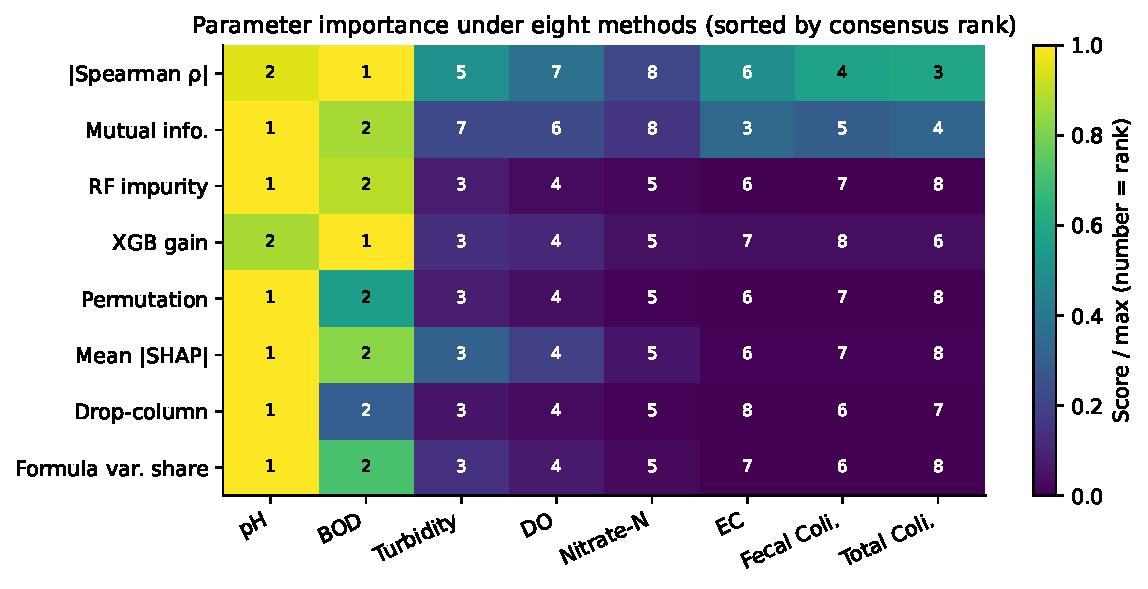
\includegraphics[width=0.95\textwidth]{fig_imp_heatmap.pdf}
  \caption{Normalised importance (colour) and rank (number) of each parameter under eight methods. The six model-based and analytic methods agree exactly on the order pH $>$ BOD $>$ turbidity $>$ DO $>$ nitrate-N. Only the two marginal-association measures (Spearman, mutual information) rank the coliforms and EC highly.}
  \label{fig:impheat}
\end{figure}

\paragraph{Agreement.} All six methods that measure a parameter's \emph{contribution to the prediction} give the same top-five order: pH, BOD, turbidity, DO, nitrate-N. These are RF impurity, XGBoost gain, permutation, SHAP, drop-column and the analytic variance share. The order matches the analytic decomposition of the formula exactly, which validates the ML-based measures: they recover the known structure.

\paragraph{Correlation is not importance.} Spearman correlation and mutual information rank fecal and total coliform third and fourth, ahead of turbidity and DO, with $\rho_S\approx0.38$. Yet removing either coliform from the full model costs no measurable \R{} (drop-column $<10^{-4}$). The coliforms correlate with the index only because sewage raises BOD and coliforms together (\cref{fig:corr}). Their information is redundant given BOD, and their own weight in the formula is negligible. Selecting parameters by correlation alone, as is common in the literature, would therefore have picked the wrong subsets.

\begin{figure}[t]
  \centering
  \begin{subfigure}[t]{0.49\textwidth}
    \centering
    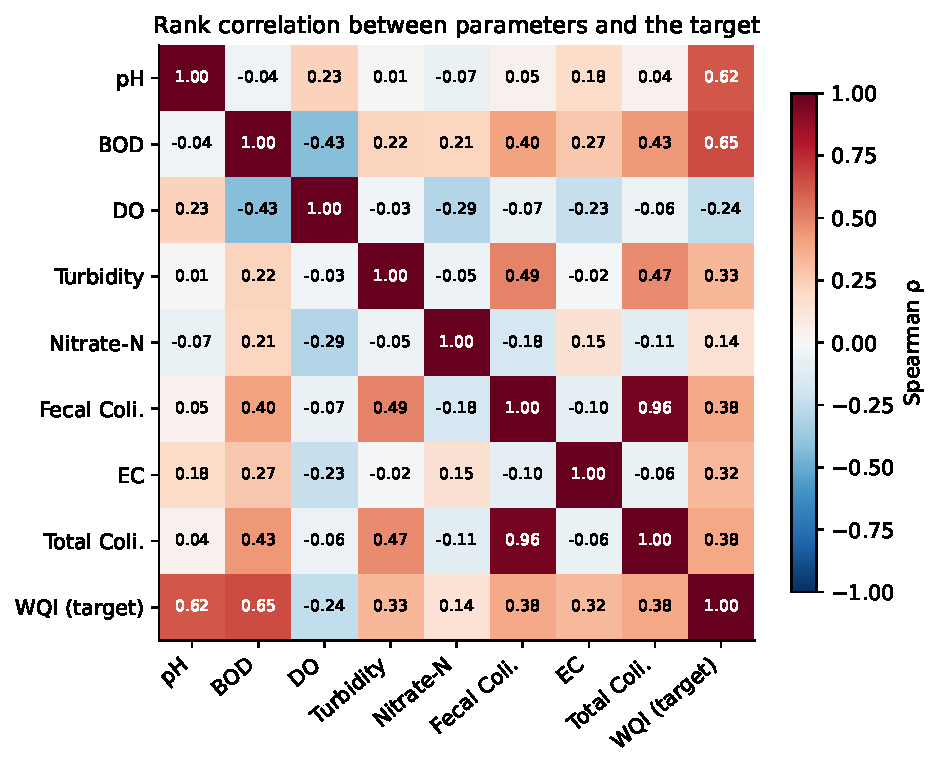
\includegraphics[width=\textwidth]{fig_imp_correlation.pdf}
    \caption{Spearman correlations.}
    \label{fig:corr}
  \end{subfigure}\hfill
  \begin{subfigure}[t]{0.49\textwidth}
    \centering
    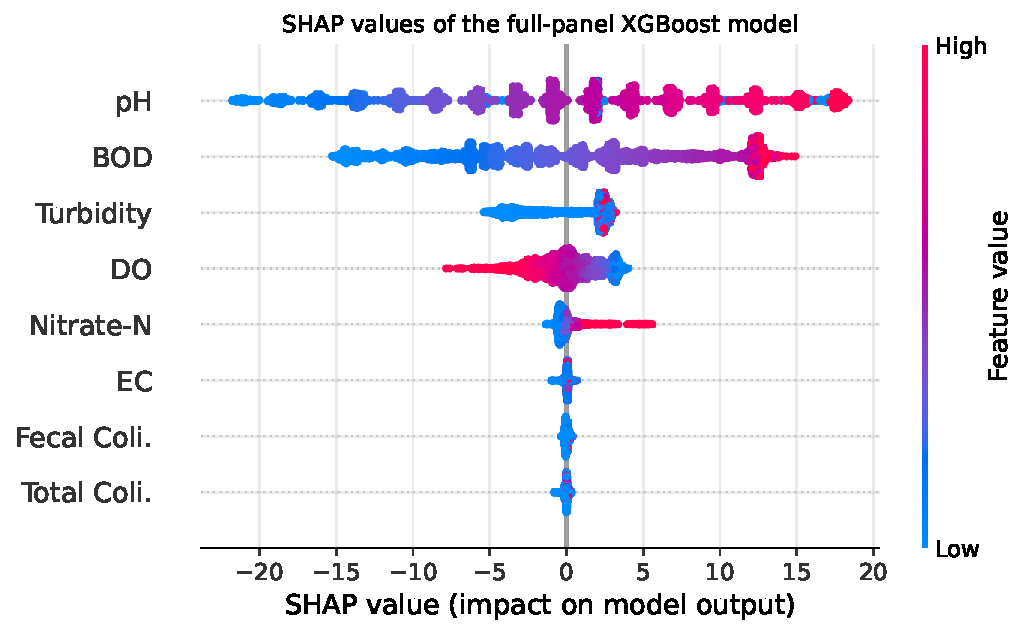
\includegraphics[width=\textwidth]{fig_imp_shap_beeswarm.pdf}
    \caption{SHAP values of the full model.}
    \label{fig:shap}
  \end{subfigure}
  \caption{(a) BOD, fecal and total coliform, turbidity and EC form a correlated ``pollution'' block ($\rho_S=0.3$--0.8), which explains why the coliforms correlate with the index without contributing to it. (b) High pH and high BOD push the prediction up by up to $\sim$20 points; the coliforms and EC have SHAP values near zero for every visit.}
\end{figure}

\paragraph{The model recovers the formula's shape.} The SHAP dependence plots\optref{fig:shapdep} show the piecewise-linear capped sub-indices: a V-shape around pH 7 that is steeper below 7 (the asymmetric band), and a linear rise in BOD that saturates at 3 mg/L (the cap at $q=100$). Turbidity likewise saturates at 10 NTU, and DO falls linearly.

\iffull
\begin{figure}[t]
  \centering
  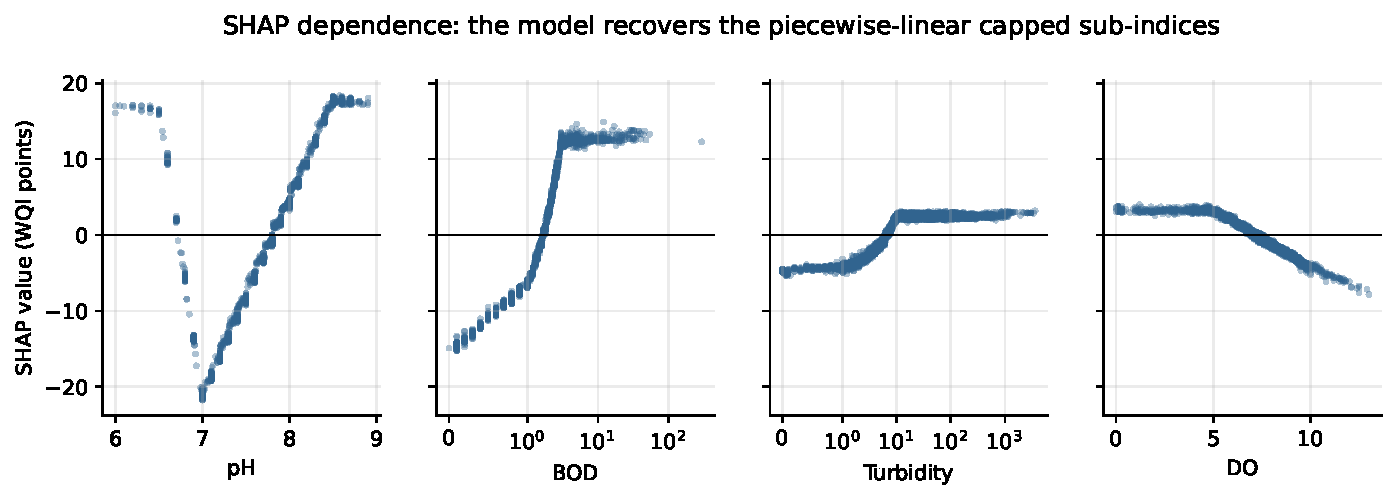
\includegraphics[width=\textwidth]{fig_imp_shap_dependence.pdf}
  \caption{SHAP dependence for the four main drivers. Saturation at BOD = 3 mg/L and turbidity = 10 NTU is the sub-index cap; the asymmetric V around pH 7 is the CPCB 6.5--8.5 band.}
  \label{fig:shapdep}
\end{figure}
\fi

\paragraph{Forward selection}\optref{fig:forward} adds parameters in exactly the consensus order. \R{} rises 0.508 (pH) $\to$ 0.939 (+BOD) $\to$ 0.977 (+turbidity) $\to$ 0.993 (+DO) $\to$ 0.998 (+nitrate-N), and adding EC and the coliforms afterwards slightly \emph{lowers} it, to 0.997, because they only add noise.

\iffull
\begin{figure}[t]
  \centering
  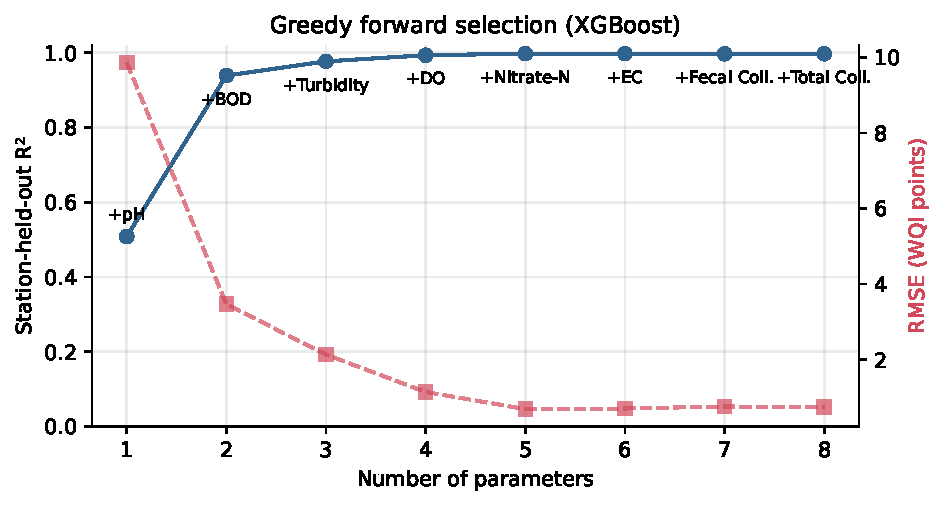
\includegraphics[width=0.72\textwidth]{fig_imp_forward_selection.pdf}
  \caption{Greedy forward selection with XGBoost on unseen stations. Five parameters reach the ceiling; the last three add nothing.}
  \label{fig:forward}
\end{figure}
\fi

\begin{keybox}[Finding 2]
The information in the CPCB index is concentrated in \textbf{pH and BOD} (\R{}\,=\,0.94 from these two alone), with \textbf{turbidity, DO and nitrate-N} completing it. Fecal coliform, total coliform and EC are statistically associated with the index but carry no usable additional information for it.
\end{keybox}

\subsection{How few parameters are enough? (RQ2)}
\label{sec:res-subsets}

\Cref{fig:comb} shows the station-held-out \R{} of all 255 subsets.

\begin{figure}[t]
  \centering
  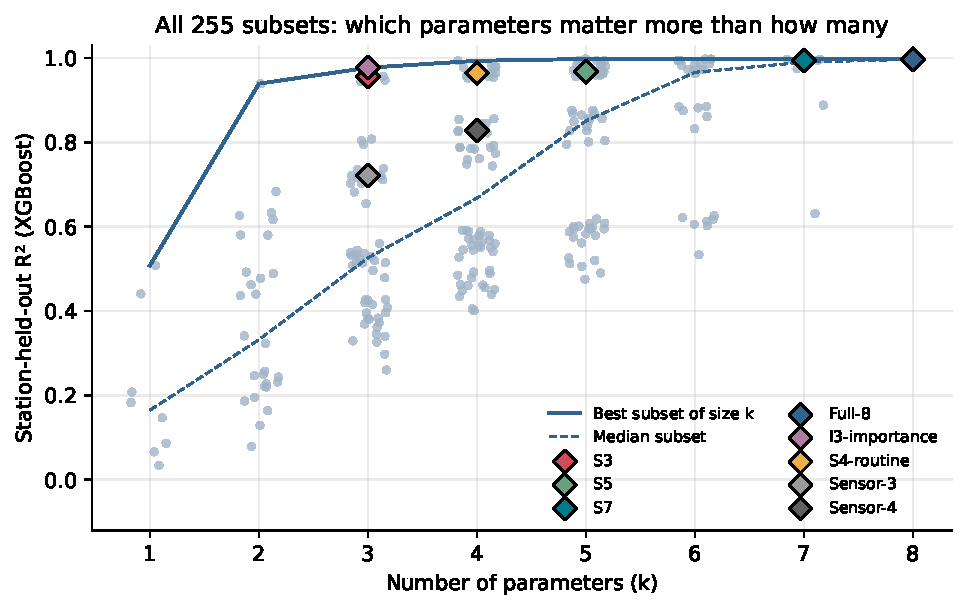
\includegraphics[width=0.85\textwidth]{fig_comb_all_subsets.pdf}
  \caption{All 255 parameter subsets (grey points, jittered) by size $k$. Solid line: best subset of each size; dashed: median. Diamonds: named subsets. At every $k\le5$ the spread between best and worst subset is far larger than the gain from adding a parameter.}
  \label{fig:comb}
\end{figure}

\paragraph{Which beats how many.} At $k=3$, \R{} ranges from 0.26 to 0.98 depending on which three parameters are chosen; at $k=4$ from 0.40 to 0.99. The \emph{best} three-parameter subset (0.977) beats the \emph{median} six-parameter subset (0.966). The ceiling is reached at $k=5$ (0.998). \Cref{tab:bestk} lists the best subset at each size\iffull, and \cref{fig:topsub} shows the top three per size\fi: every top subset contains pH and BOD.

\begin{table}[h]
\centering\small
\caption{Best subset of each size (XGBoost, unseen stations).}
\label{tab:bestk}
\begin{tabular}{rlrrr}
\toprule
$k$ & Best subset & \R{} & RMSE & Cat.\ acc. \\
\midrule
1 & pH & 0.508 & 9.86 & 68.3\% \\
2 & pH, BOD & 0.939 & 3.47 & 89.3\% \\
3 & pH, BOD, turbidity & 0.977 & 2.14 & 94.0\% \\
4 & pH, BOD, DO, turbidity & 0.993 & 1.15 & 96.8\% \\
5 & pH, BOD, DO, turbidity, nitrate-N & 0.998 & 0.69 & 97.8\% \\
6 & + EC & 0.997 & 0.73 & 97.9\% \\
7 & + fecal \& total coliform (no EC) & 0.997 & 0.74 & 97.9\% \\
8 & all & 0.997 & 0.76 & 97.8\% \\
\bottomrule
\end{tabular}
\end{table}

\iffull
\begin{figure}[t]
  \centering
  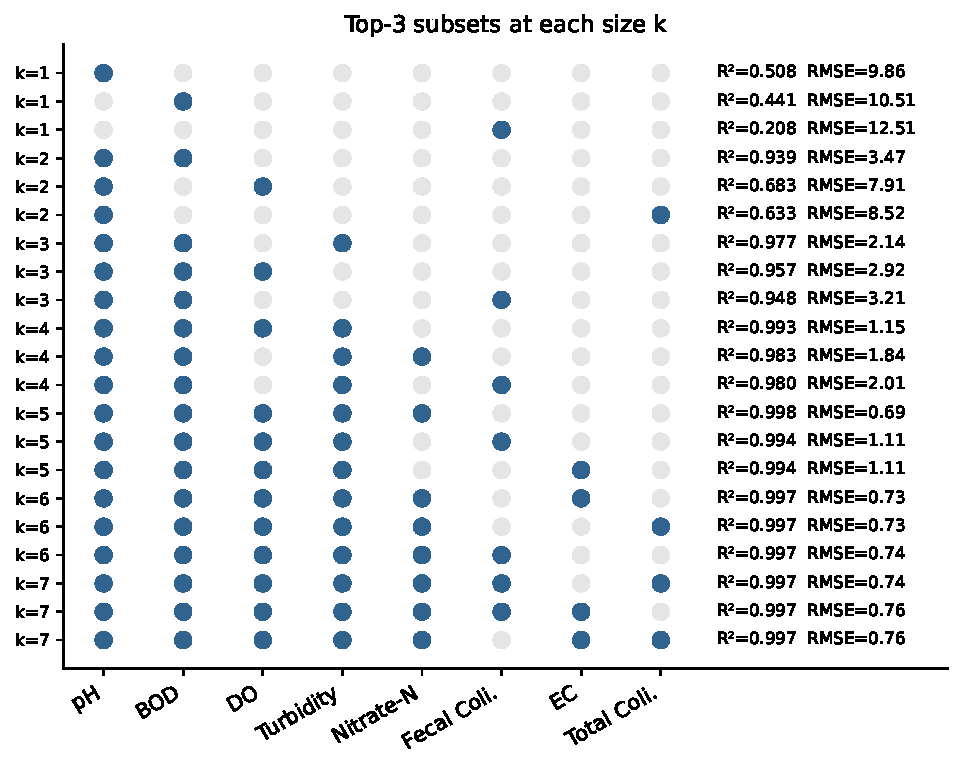
\includegraphics[width=0.78\textwidth]{fig_comb_top_subsets.pdf}
  \caption{The three best subsets at each size (filled = parameter included).}
  \label{fig:topsub}
\end{figure}
\fi

\paragraph{How the pre-registered subsets fare.} \sub{S3} (pH, DO, BOD) is the 2nd-best of 56 three-parameter subsets (\R{}\,=\,0.957), so the availability-based choice was a good one. \sub{S5} ranks only 13th of 56 five-parameter subsets: its two extra parameters, fecal coliform and EC, are the near-weightless ones. \sub{S7} ranks 4th of 8 (0.994), because it contains turbidity but misses nitrate-N. The probe-only \sub{Sensor-3} (pH, DO, EC; \R{}\,=\,0.72) and \sub{Sensor-4} (+turbidity; 0.83) are far behind, because they lack BOD, the second-largest driver of the index.

\paragraph{ML versus re-weighting the formula.} The obvious no-ML alternative is to evaluate \cref{eq:wqi} over the available parameters with renormalised weights. \iffull\Cref{fig:mlformula} compares it with XGBoost for all 255 subsets.\fi The model is better for every subset that misses a parameter with non-negligible weight, and the gap is large exactly where it matters. For \sub{S3}, \R{} is 0.863 with the formula and 0.957 with XGBoost, and RMSE falls from 5.21 to 2.93. For \sub{Sensor-4} it is 0.389 versus 0.828. The model learns the \emph{expected} contribution of the missing parameters conditional on the observed ones, while the formula implicitly assumes the missing parameters behave like the observed ones. Only when the missing parameters are the weightless coliforms and EC (\sub{I5}, \sub{Full-8}) is the formula essentially exact, since then nothing is missing that matters.

\iffull
\begin{figure}[t]
  \centering
  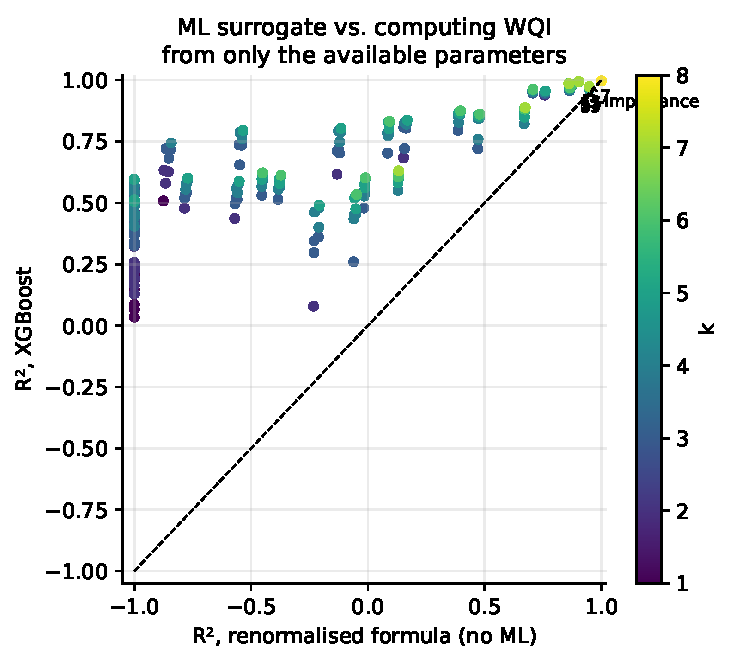
\includegraphics[width=0.55\textwidth]{fig_comb_ml_vs_formula.pdf}
  \caption{\R{} of XGBoost against \R{} of the renormalised formula, for every subset (colour = $k$). Points above the diagonal are subsets where learning beats re-weighting; that is almost all of them.}
  \label{fig:mlformula}
\end{figure}
\fi

\subsection{Model comparison}
\label{sec:res-models}

\Cref{fig:heat} shows \R{} for every model and subset, and \cref{tab:xgbmain} gives the full metrics for the best model, XGBoost.

\begin{figure}[t]
  \centering
  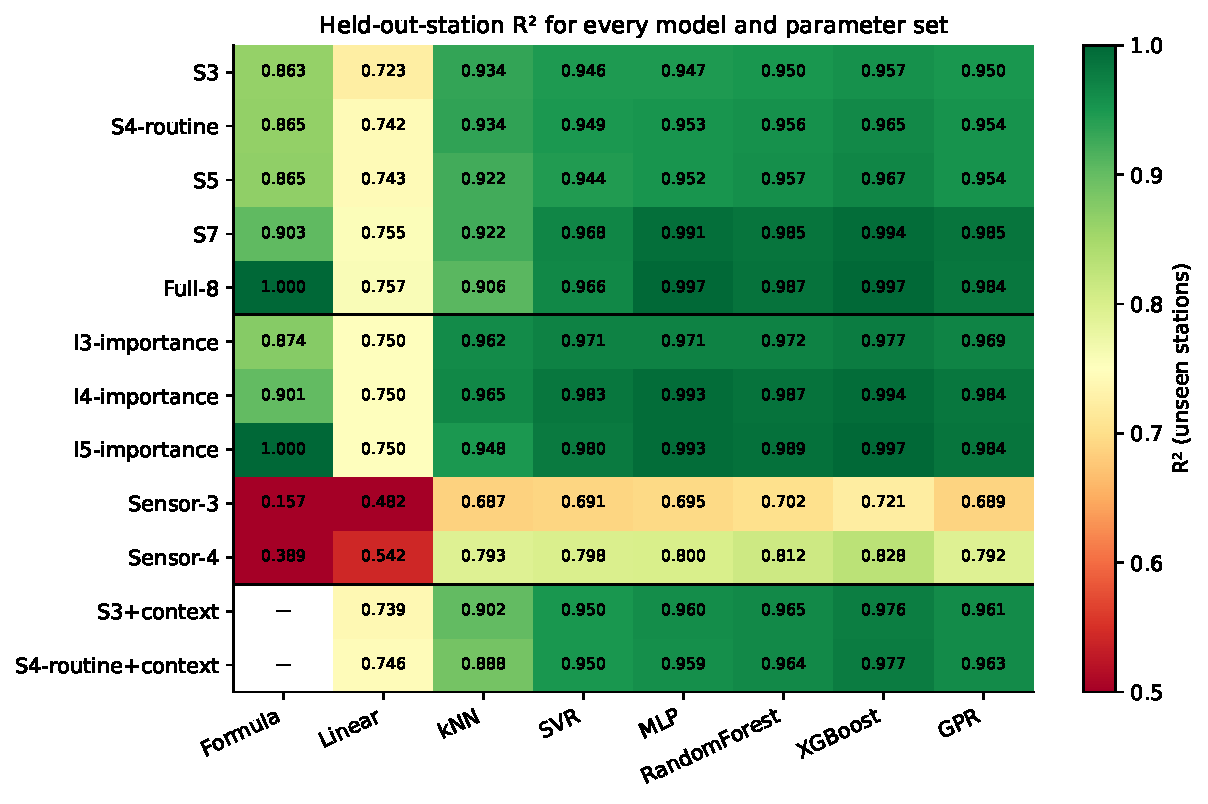
\includegraphics[width=0.9\textwidth]{fig_models_r2_heatmap.pdf}
  \caption{Station-held-out \R{} for 8 models $\times$ 12 subsets. Rows: pre-registered/routine subsets (top), importance and sensor subsets (middle), subsets with location and month context (bottom).}
  \label{fig:heat}
\end{figure}

\begin{table}[t]
\centering\small
\caption{XGBoost on unseen stations (mean $\pm$ s.d.\ across the 5 folds for \R{}, RMSE and category accuracy). ``$\pm$5'' = share of predictions within 5 WQI points. No reduced-parameter prediction was ever two or more categories away from the truth.}
\label{tab:xgbmain}
\begin{tabular}{lrrrrrrr}
\toprule
Subset & $k$ & \R{} (=NSE) & RMSE & MAE & KGE & Cat.\ acc. & $\pm$5 \\
\midrule
\sub{S3} & 3 & 0.957 $\pm$ .006 & 2.93 $\pm$ .11 & 2.42 & 0.968 & 90.6 $\pm$ 0.3\% & 92.3\% \\
\sub{S4-routine} & 4 & 0.965 $\pm$ .004 & 2.65 $\pm$ .10 & 2.07 & 0.970 & 91.8 $\pm$ 0.8\% & 94.0\% \\
\sub{S5} & 5 & 0.967 $\pm$ .004 & 2.56 $\pm$ .08 & 1.96 & 0.971 & 92.3 $\pm$ 1.0\% & 94.1\% \\
\sub{S7} & 7 & 0.994 $\pm$ .001 & 1.08 $\pm$ .07 & 0.70 & 0.989 & 97.0 $\pm$ 1.2\% & 99.3\% \\
\sub{Full-8} & 8 & 0.997 $\pm$ .001 & 0.76 $\pm$ .05 & 0.53 & 0.990 & 97.8 $\pm$ 0.6\% & 99.9\% \\
\midrule
\sub{I3-importance} & 3 & 0.977 $\pm$ .003 & 2.14 $\pm$ .08 & 1.58 & 0.980 & 94.0 $\pm$ 1.2\% & 97.1\% \\
\sub{I4-importance} & 4 & 0.994 $\pm$ .001 & 1.13 $\pm$ .10 & 0.74 & 0.988 & 96.8 $\pm$ 1.0\% & 99.3\% \\
\sub{I5-importance} & 5 & 0.998 $\pm$ .000 & 0.70 $\pm$ .04 & 0.49 & 0.990 & 97.7 $\pm$ 0.7\% & 99.9\% \\
\sub{Sensor-3} & 3 & 0.721 $\pm$ .040 & 7.42 $\pm$ .41 & 5.81 & 0.797 & 77.5 $\pm$ 1.1\% & 52.8\% \\
\sub{Sensor-4} & 4 & 0.828 $\pm$ .022 & 5.82 $\pm$ .25 & 4.46 & 0.875 & 82.4 $\pm$ 0.9\% & 64.9\% \\
\midrule
\sub{S3+context} & 7 & 0.976 $\pm$ .003 & 2.17 $\pm$ .04 & 1.58 & 0.977 & 93.3 $\pm$ 0.8\% & 96.5\% \\
\sub{S4-routine+context} & 8 & 0.977 $\pm$ .003 & 2.12 $\pm$ .02 & 1.55 & 0.978 & 93.9 $\pm$ 0.8\% & 96.7\% \\
\bottomrule
\end{tabular}
\end{table}

\paragraph{Ranking of models.} XGBoost is the best or joint-best model for every subset. Random forest, MLP and GPR follow within 0.005--0.01 \R{} on the reduced subsets, and SVR and $k$NN a little further behind. The model family matters far less than the parameter subset: for \sub{S3}, the five flexible models span \R{}\,=\,0.934--0.957, whereas changing the subset at fixed model spans 0.72--0.998. Two models are clearly unsuitable:
\begin{itemize}
  \item \textbf{Linear regression} (\R{}\,$\approx$\,0.72--0.76 for every subset) cannot represent the piecewise-linear, capped, V-shaped sub-indices, especially after the log transforms. It is worse than the plain formula wherever the formula has the relevant parameters.
  \item \textbf{$k$NN} degrades as parameters are \emph{added} (0.934 for \sub{S3} to 0.906 for \sub{Full-8}). The uninformative coliform and EC dimensions dilute its distance metric, a textbook curse-of-dimensionality effect.
\end{itemize}

\paragraph{Accuracy versus parameter count}\optref{fig:vssubset}. For the flexible models, RMSE falls only slightly from \sub{S3} to \sub{S5} (2.93 $\to$ 2.56 for XGBoost) and then sharply at \sub{S7} (1.08), the first pre-registered subset to include turbidity. Category accuracy follows the same pattern: 90.6\%, 91.8\%, 92.3\%, 97.0\%, 97.8\%. Every reduced model is far above the 58\% majority baseline.

\iffull
\begin{figure}[t]
  \centering
  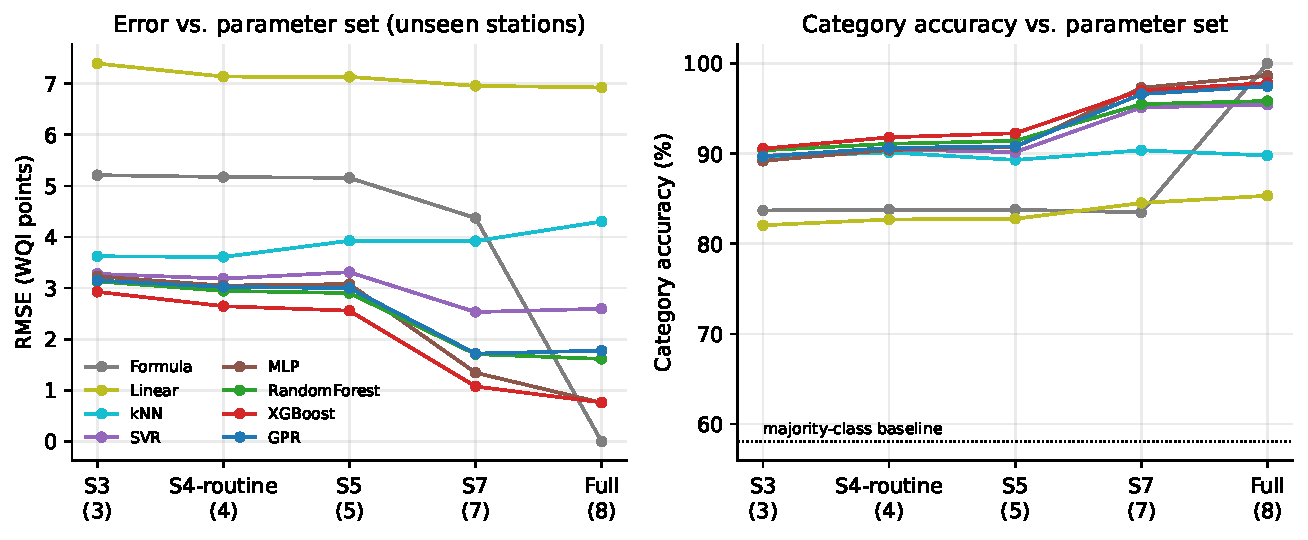
\includegraphics[width=\textwidth]{fig_models_vs_subset.pdf}
  \caption{RMSE (left) and category accuracy (right) against the pre-registered subsets, for each model. The formula reaches zero error only at \sub{Full-8}, where it \emph{is} the target.}
  \label{fig:vssubset}
\end{figure}
\fi

\paragraph{What the errors look like.} \Cref{fig:predtrue} plots predictions against the truth. The \sub{S3} model shows mild regression to the mean: it slightly over-predicts clean sites and under-predicts the worst. The confusion matrices\optref{fig:confusion} show that all category errors occur between adjacent classes, mostly Good$\leftrightarrow$Poor. \Cref{fig:s3resid} explains the \sub{S3} error. Its residual is almost exactly the negative of the unseen parameters' contribution to the index ($r=-0.81$). The model fills in the \emph{average} turbidity/nitrate contribution of about 6 points, so its error is largest when turbidity is atypically low (clear water) or capped (silt-laden water).

\begin{figure}[t]
  \centering
  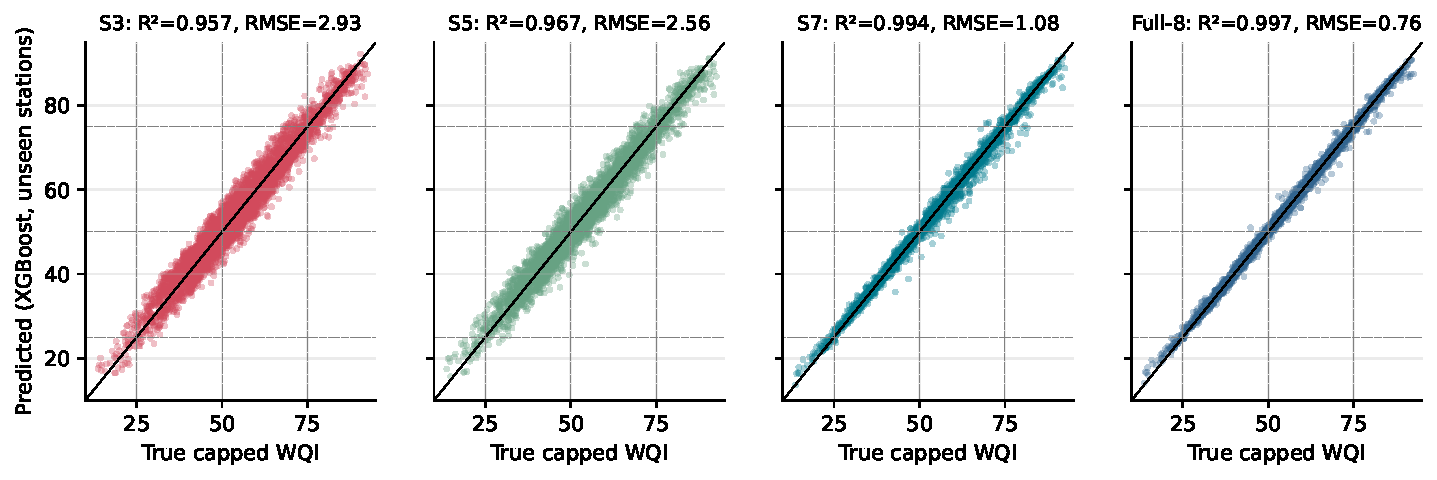
\includegraphics[width=\textwidth]{fig_models_pred_vs_true.pdf}
  \caption{Predicted against true WQI for XGBoost on unseen stations. Dashed lines are category boundaries.}
  \label{fig:predtrue}
\end{figure}

\iffull
\begin{figure}[t]
  \centering
  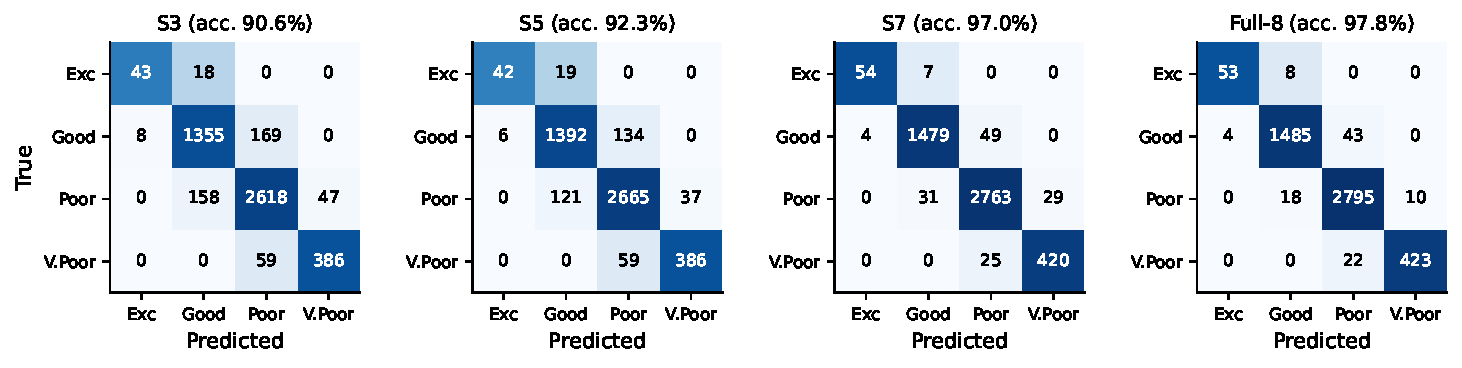
\includegraphics[width=\textwidth]{fig_models_confusion.pdf}
  \caption{Category confusion matrices (counts) for XGBoost on unseen stations. Every error is to an adjacent category.}
  \label{fig:confusion}
\end{figure}
\fi

\begin{figure}[t]
  \centering
  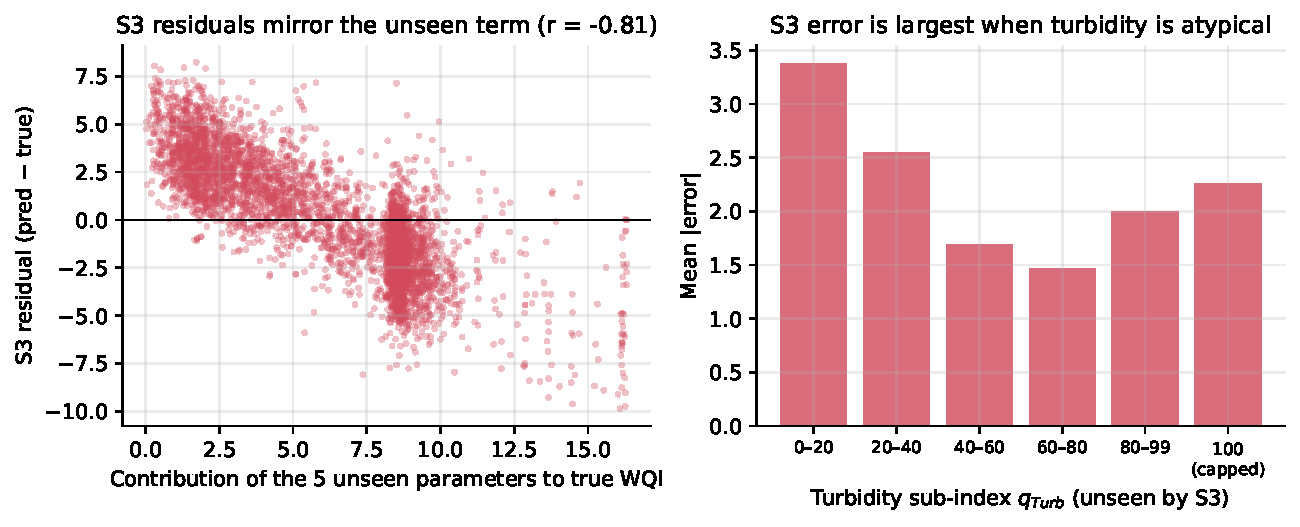
\includegraphics[width=0.95\textwidth]{fig_models_s3_residuals.pdf}
  \caption{Anatomy of the \sub{S3} error. Left: residual against the true contribution of the five unseen parameters. Right: mean absolute error by turbidity sub-index.}
  \label{fig:s3resid}
\end{figure}

\paragraph{Location and season as free extra inputs.} Adding latitude, longitude and month, which every station knows for free, raises \sub{S3} from \R{}\,=\,0.957 to 0.976 (RMSE 2.93 $\to$ 2.17) and \sub{S4-routine} to 0.977. That is almost exactly what measuring turbidity instead of DO achieves (\sub{I3}, 0.977), at zero measurement cost. The context features let the model learn where and when turbidity is typically high: monsoon months, and the silt-laden rivers of the Indo-Gangetic plain. This is achieved on \emph{unseen stations}, so the model is learning regional and seasonal patterns, not memorising stations.

\subsection{Generalisation beyond the training stations}
\label{sec:res-general}

\Cref{tab:schemes}\iffull{} and \cref{fig:general}\fi{} compare the five validation schemes.

\begin{table}[h]
\centering\small
\caption{XGBoost \R{} / RMSE under the five validation schemes.}
\label{tab:schemes}
\begin{tabular}{lccccc}
\toprule
Subset & Random rows & Unseen stations & Unseen rivers & Unseen states & Unseen season \\
\midrule
\sub{S3} & 0.958 / 2.87 & 0.957 / 2.93 & 0.942 / 3.38 & 0.943 / 3.35 & 0.949 / 3.18 \\
\sub{S4-routine} & 0.967 / 2.57 & 0.965 / 2.65 & 0.947 / 3.25 & 0.941 / 3.41 & 0.957 / 2.93 \\
\sub{S5} & 0.969 / 2.46 & 0.967 / 2.56 & 0.948 / 3.21 & 0.942 / 3.40 & 0.959 / 2.85 \\
\sub{S7} & 0.995 / 1.03 & 0.994 / 1.08 & 0.991 / 1.31 & 0.990 / 1.41 & 0.993 / 1.20 \\
\sub{Full-8} & 0.997 / 0.73 & 0.997 / 0.76 & 0.995 / 0.95 & 0.995 / 0.99 & 0.996 / 0.85 \\
\sub{I3-importance} & 0.978 / 2.09 & 0.977 / 2.14 & 0.969 / 2.47 & 0.967 / 2.54 & 0.974 / 2.28 \\
\sub{I5-importance} & 0.998 / 0.66 & 0.998 / 0.70 & 0.996 / 0.84 & 0.996 / 0.86 & 0.997 / 0.79 \\
\bottomrule
\end{tabular}
\end{table}

\iffull
\begin{figure}[t]
  \centering
  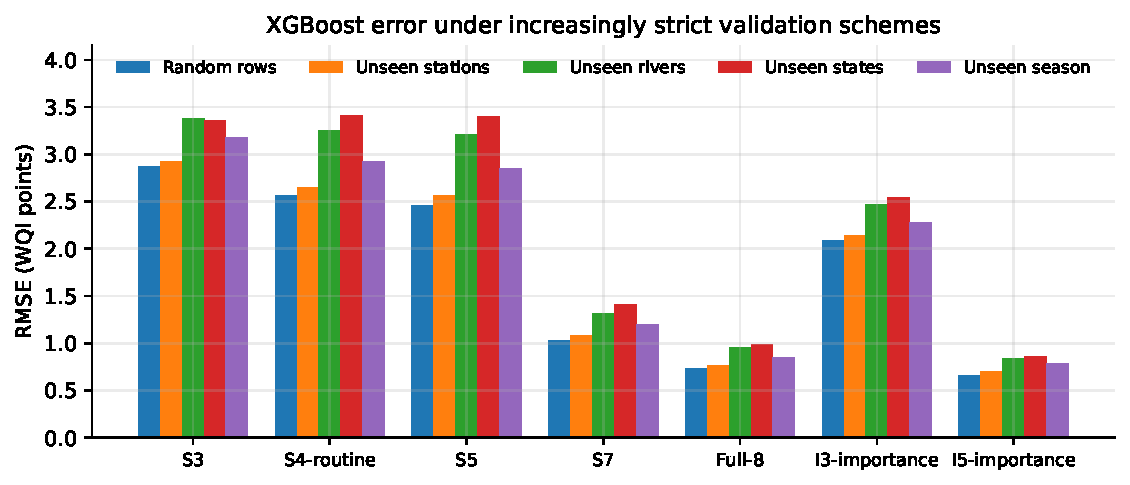
\includegraphics[width=0.92\textwidth]{fig_models_generalisation.pdf}
  \caption{XGBoost RMSE under increasingly strict validation. Holding out whole rivers or states costs \sub{S3} about 0.4--0.5 WQI points.}
  \label{fig:general}
\end{figure}
\fi

Three observations follow.
\begin{enumerate}
  \item \textbf{Random splits are only mildly optimistic here.} For \sub{S3}, RMSE is 2.87 with random rows and 2.93 with unseen stations. The relationship being learned is mostly physico-chemical rather than station-specific, so station memorisation buys little. This is a property of this target, not a licence to use random splits in general.
  \item \textbf{Transfer to unseen rivers and states costs 15\%.} \sub{S3} RMSE rises from 2.93 to 3.35--3.38, and category accuracy falls from 90.6\% to 89.2--89.6\%. Even with the whole river, or whole states, held out, \R{} stays above 0.94.
  \item \textbf{Seasonal transfer is intermediate.} Training without the monsoon (or any other season) and predicting it gives \R{}\,=\,0.949 for \sub{S3}. Because the full panel exists only for 2020, this is the strongest temporal test the data permit.
\end{enumerate}

Station density matters little\optref{tab:density}. Stations with only 1--3 visits are predicted about as well as stations with 10--12, which is encouraging for sparsely monitored sites.

\iffull
\begin{table}[h]
\centering\small
\caption{Mean absolute error (XGBoost, unseen stations) by number of labelled visits at the station.}
\label{tab:density}
\begin{tabular}{lrrrrrr}
\toprule
Visits per station & Rows & \sub{S3} & \sub{S5} & \sub{S7} & \sub{Full-8} & \sub{I3} \\
\midrule
1--3 & 177 & 2.40 & 2.24 & 0.97 & 0.74 & 1.81 \\
4--6 & 580 & 2.50 & 2.53 & 0.82 & 0.65 & 1.59 \\
7--9 & 1,148 & 2.41 & 2.17 & 0.70 & 0.57 & 1.58 \\
10--12 & 2,126 & 2.69 & 2.08 & 0.71 & 0.49 & 1.50 \\
13+ & 830 & 1.69 & 0.91 & 0.55 & 0.47 & 1.75 \\
\bottomrule
\end{tabular}
\end{table}
\fi
